% -*- TeX-engine: xetex; eval: (auto-fill-mode 0); eval: (visual-line-mode 1); -*-
% Compile with XeLaTeX

%%%%%%%%%%%%%%%%%%%%%%%
% Option 1: Slides: (comment for handouts)   %
%%%%%%%%%%%%%%%%%%%%%%%

\documentclass[slidestop,compress,mathserif,12pt,t,professionalfonts,xcolor=table]{beamer}

% solution stuff
\newcommand{\solnMult}[1]{
\only<1>{#1}
\only<2->{\red{\textbf{#1}}}
}
\newcommand{\soln}[1]{\textit{#1}}

%%%%%%%%%%%%%%%%%%%%%%%%%%%%%%%
% Option 2: Handouts, without solutions (post before class)    %
%%%%%%%%%%%%%%%%%%%%%%%%%%%%%%%

% \documentclass[11pt,containsverbatim,handout,xcolor=xelatex,dvipsnames,table]{beamer}

% % handout layout
% \usepackage{pgfpages}
% \pgfpagesuselayout{4 on 1}[letterpaper,landscape,border shrink=5mm]

% % solution stuff
% \newcommand{\solnMult}[1]{#1}
% \newcommand{\soln}[1]{}

%%%%%%%%%%%%%%%%%%%%%%%%%%%%%%%%%%%%
% Option 3: Handouts, with solutions (may post after class if need be)    %
%%%%%%%%%%%%%%%%%%%%%%%%%%%%%%%%%%%%

% \documentclass[11pt,containsverbatim,handout,xcolor=xelatex,dvipsnames,table]{beamer}

% % handout layout
% \usepackage{pgfpages}
% \pgfpagesuselayout{4 on 1}[letterpaper,landscape,border shrink=5mm]

% % solution stuff
% \newcommand{\solnMult}[1]{\red{\textbf{#1}}}
% \newcommand{\soln}[1]{\textit{#1}}

%%%%%%%%%%
% Load style file, defaults  %
%%%%%%%%%%

%%%%%%%%%%%%%%%%
% Themes
%%%%%%%%%%%%%%%%

% See http://deic.uab.es/~iblanes/beamer_gallery/ for mor options

% Style theme
\usetheme{Pittsburgh}

% Color theme
\usecolortheme{seahorse}

% Helvetica Neue Light for most text
\usepackage{fontspec}
\setsansfont{Helvetica Neue Light}

%%%%%%%%%%%%%%%%
% Packages
%%%%%%%%%%%%%%%%

\usepackage{geometry}
\usepackage{graphicx}
\usepackage{amssymb}
\usepackage{epstopdf}
\usepackage{amsmath}  	% this permits text in eqnarray among other benefits
\usepackage{url}		% produces hyperlinks
\usepackage[english]{babel}
\usepackage{colortbl}	% allows for color usage in tables
\usepackage{multirow}	% allows for rows that span multiple rows in tables
\usepackage{color}		% this package has a variety of color options
\usepackage{pgf}
\usepackage{calc}
\usepackage{ulem}
\usepackage{multicol}
\usepackage{textcomp}
\usepackage{listings}
\usepackage{changepage}
\usepackage{tikz}
\usetikzlibrary{trees}		% for probability trees
\usepackage{fancyvrb}	% for colored code chunks
\usepackage{nameref}

%%%%%%%%%%%%%%%%
% Remove navigation symbols
%%%%%%%%%%%%%%%%

\beamertemplatenavigationsymbolsempty
\hypersetup{pdfpagemode=UseNone} % don't show bookmarks on initial view

%%%%%%%%%%%%%%%%
% User defined colors
%%%%%%%%%%%%%%%%

% Pantone 2016 Spring colors
% https://atelierbram.github.io/c-tiles16/colorscheming/pantone-spring-2016-colortable.html
% update each semester or year

\xdefinecolor{custom_blue}{rgb}{0.01, 0.31, 0.52} % Snorkel Blue
\xdefinecolor{custom_darkBlue}{rgb}{0.20, 0.20, 0.39} % Reflecting Pond  
\xdefinecolor{custom_orange}{rgb}{0.96, 0.57, 0.42} % Cadmium Orange
\xdefinecolor{custom_green}{rgb}{0, 0.47, 0.52} % Biscay Bay
\xdefinecolor{custom_red}{rgb}{0.58, 0.32, 0.32} % Marsala

\xdefinecolor{custom_lightGray}{rgb}{0.78, 0.80, 0.80} % Glacier Gray
\xdefinecolor{custom_darkGray}{rgb}{0.35, 0.39, 0.43} % Stormy Weather

%%%%%%%%%%%%%%%%
% Template colors
%%%%%%%%%%%%%%%%

\setbeamercolor*{palette primary}{fg=white,bg= custom_blue}
\setbeamercolor*{palette secondary}{fg=black,bg= custom_blue!80!black}
\setbeamercolor*{palette tertiary}{fg=white,bg= custom_blue!80!black!80}
\setbeamercolor*{palette quaternary}{fg=white,bg= custom_blue}

\setbeamercolor{structure}{fg= custom_blue}
\setbeamercolor{frametitle}{bg= custom_blue!90}
\setbeamertemplate{blocks}[shadow=false]
\setbeamersize{text margin left=2em,text margin right=2em}

%%%%%%%%%%%%%%%%
% Styling fonts, bullets, etc.
%%%%%%%%%%%%%%%%

% title slide
\setbeamerfont{title}{size=\large,series=\bfseries}
\setbeamerfont{subtitle}{size=\large,series=\mdseries}
%\setbeamerfont{institute}{size=\large,series=\mdseries}

% color of alerted text
\setbeamercolor{alerted text}{fg=custom_orange}

% styling of itemize bullets
\setbeamercolor{item}{fg=custom_blue}
\setbeamertemplate{itemize item}{{{\small$\blacktriangleright$}}}
\setbeamercolor{subitem}{fg=custom_blue}
\setbeamertemplate{itemize subitem}{{\textendash}}
\setbeamerfont{itemize/enumerate subbody}{size=\footnotesize}
\setbeamerfont{itemize/enumerate subitem}{size=\footnotesize}

% styling of enumerate bullets
\setbeamertemplate{enumerate item}{\insertenumlabel.}
\setbeamerfont{enumerate item}{family={\fontspec{Helvetica Neue}}}
\setbeamerfont{enumerate subitem}{family={\fontspec{Helvetica Neue}}}
\setbeamerfont{enumerate subsubitem}{family={\fontspec{Helvetica Neue}}}

% make frame titles small to make room in the slide
\setbeamerfont{frametitle}{size=\small} 

% set Helvetica Neue font for frame and section titles
\setbeamerfont{frametitle}{family={\fontspec{Helvetica Neue}}}
\setbeamerfont{sectiontitle}{family={\fontspec{Helvetica Neue}}}
\setbeamerfont{section in toc}{family={\fontspec{Helvetica Neue}}}
\setbeamerfont{subsection in toc}{family={\fontspec{Helvetica Neue}}, size=\small}
\setbeamerfont{footline}{family={\fontspec{Helvetica Neue}}}
\setbeamerfont{subsection in toc}{family={\fontspec{Helvetica Neue}}}
\setbeamerfont{block title}{family={\fontspec{Helvetica Neue}}}

%%%%%%%%%%%%%%%%
% New fonts accessed by fontspec package
%%%%%%%%%%%%%%%%

% Monaco font for code
\newfontfamily{\monaco}{Monaco}

%%%%%%%%%%%%%%%%
% Color text commands
%%%%%%%%%%%%%%%%

%orange
\newcommand{\orange}[1]{\textit{\textcolor{custom_orange}{#1}}}

% yellow
\newcommand{\yellow}[1]{\textit{\textcolor{yellow}{#1}}}

% blue
\newcommand{\blue}[1]{\textit{\textcolor{blue}{#1}}}

% green
\newcommand{\green}[1]{\textit{\textcolor{custom_green}{#1}}}

% red
\newcommand{\red}[1]{\textit{\textcolor{custom_red}{#1}}}

% dark gray
\newcommand{\darkgray}[1]{\textit{\textcolor{custom_darkGray}{#1}}}

% light gray
\newcommand{\lightgray}[1]{\textit{\textcolor{custom_lightGray}{#1}}}

% pink
\newcommand{\pink}[1]{\textit{\textcolor{pink}{#1}}}


%%%%%%%%%%%%%%%%
% Custom commands
%%%%%%%%%%%%%%%%

% empty box for probability tree frame
\newcommand{\emptybox}[2]{
	\fbox{ \begin{minipage}{#1} \hfill\vspace{#2} \end{minipage} }
}

% cancel
\newcommand{\cancel}[1]{%
    \tikz[baseline=(tocancel.base)]{
        \node[inner sep=0pt,outer sep=0pt] (tocancel) {#1};
        \draw[red, line width=0.5mm] (tocancel.south west) -- (tocancel.north east);
    }%
}

% degree
\newcommand{\degree}{\ensuremath{^\circ}}

% cite
\newcommand{\ct}[1]{
\vfill
{\tiny #1}}

% Note
\newcommand{\Note}[1]{
\rule{2.5cm}{0.25pt} \\ \textit{\footnotesize{\textcolor{custom_red}{Note:} \textcolor{custom_darkGray}{#1}}}}

% Remember
\newcommand{\Remember}[1]{\textit{\scriptsize{\textcolor{custom_red}{Remember:} #1}}}

% links: webURL, webLink
\newcommand{\webURL}[1]{\urlstyle{same}{\textit{\textcolor{custom_blue}{\url{#1}}}}}
\newcommand{\webLink}[2]{\href{#1}{\textcolor{custom_blue}{{#2}}}}

% mail
\newcommand{\mail}[1]{\href{mailto:#1}{\textit{\textcolor{custom_blue}{#1}}}}

% highlighting: hl, hlGr, mathhl
\newcommand{\hl}[1]{\textit{\textcolor{custom_blue}{#1}}}
\newcommand{\hlGr}[1]{\textit{\textcolor{custom_green}{#1}}}
\newcommand{\mathhl}[1]{\textcolor{custom_blue}{\ensuremath{#1}}}

% example
\newcommand{\ex}[1]{\textcolor{blue}{{{\small (#1)}}}}

% twocol: two columns
\newenvironment{twocol}[4]{
\begin{columns}[c]
\column{#1\textwidth}
#3
\column{#2\textwidth}
#4
\end{columns}
}

% threecol: three columns
\newenvironment{threecol}[6]{
\begin{columns}[c]
\column{#1\textwidth}
#4
\column{#2\textwidth}
#5
\column{#3\textwidth}
#6
\end{columns}
}

% slot (for probability calculations)
\newenvironment{slot}[2]{
\begin{array}{c} 
\underline{#1} \\ 
#2
\end{array}
}

% pr: left and right parentheses
\newcommand{\pr}[1]{
\left( #1 \right)
}

%%%%%%%%%%%%%%%%
% Custom blocks
%%%%%%%%%%%%%%%%

% activity: less commonly used
\newcommand{\activity}[2]{
\setbeamertemplate{itemize item}{{{\small\textcolor{custom_orange}{$\blacktriangleright$}}}}
\setbeamercolor{block title}{fg=white, bg=custom_orange}
\setbeamerfont{block title}{size=\small}
\setbeamercolor{block body}{fg=black, bg=custom_orange!20!white!80}
\setbeamerfont{block body}{size=\small}
\begin{block}{Activity: #1}
\setlength\abovedisplayskip{0pt}
#2
\end{block}
}

% app: application exercise
\newcommand{\app}[2]{
\setbeamercolor{block title}{fg=white,bg=custom_green}
\setbeamercolor{block body}{fg=black,bg=custom_green!20!white!80}
\begin{block}{{\small Application exercise: #1}}
#2
\end{block}
}

% disc: discussion question
\newcommand{\disc}[1]{
\vspace*{-2ex}
\setbeamercolor{block body}{bg=custom_blue!25!white!80, fg=custom_blue!55!black!95}
\begin{block}{\vspace*{-3ex}}
#1
\end{block}
\vspace*{-1ex}
}

% clicker: clicker question
\newcommand{\clicker}[1]{
\setbeamercolor{block title}{bg=custom_blue!80!white!50,fg=custom_blue!30!black!90}
\setbeamercolor{block body}{bg=custom_blue!20!white!80,fg=custom_blue!30!black!90}
\begin{block}{\vspace*{-0.2ex}{\footnotesize Clicker question}\vspace*{-0.2ex}}
#1
\end{block}
}

% formula
\newcommand{\formula}[2]{
\setbeamercolor{block title}{bg=custom_blue!40!white!60,fg=custom_blue!55!black!95}
\begin{block}{{\small#1}}
#2
\end{block}
}

% code
\newcommand{\Rcode}[1]{
{\monaco {\footnotesize \textcolor{custom_darkBlue}{#1}}}
}

% output
\newcommand{\Rout}[1]{
{\monaco {\footnotesize \textcolor{custom_darkGray}{#1}}}
}

%%%%%%%%%%%%%%%%
% Change margin
%%%%%%%%%%%%%%%%

\newenvironment{changemargin}[2]{%
\begin{list}{}{%
\setlength{\topsep}{0pt}%
\setlength{\leftmargin}{#1}%
\setlength{\rightmargin}{#2}%
\setlength{\listparindent}{\parindent}%
\setlength{\itemindent}{\parindent}%
\setlength{\parsep}{\parskip}%
}%
\item}{\end{list}}

%%%%%%%%%%%%%%%%
% Footnote
%%%%%%%%%%%%%%%%

\long\def\symbolfootnote[#1]#2{\begingroup%
\def\thefootnote{\fnsymbol{footnote}}\footnote[#1]{#2}\endgroup}

%%%%%%%%%%%%%%%%
% Graphics
%%%%%%%%%%%%%%%%

\DeclareGraphicsRule{.tif}{png}{.png}{`convert #1 `dirname #1`/`basename #1 .tif`.png}

%%%%%%%%%%%%%%%%
% Slide number
%%%%%%%%%%%%%%%%

\setbeamertemplate{footline}{%
    \raisebox{5pt}{\makebox[\paperwidth]{\hfill\makebox[20pt]{\color{gray}
          \scriptsize\insertframenumber}}}\hspace*{5pt}}

          
%%%%%%%%%%%%%%%%
% Remove page numbers
%%%%%%%%%%%%%%%%

\newcommand{\removepagenumbers}{% 
  \setbeamertemplate{footline}{}
}

%%%%%%%%%%%%%%%%
% TOC slides
%%%%%%%%%%%%%%%%

\setbeamertemplate{section in toc}{\inserttocsectionnumber.~\inserttocsection}
\setbeamertemplate{subsection in toc}{$\qquad$\inserttocsubsectionnumber.~\inserttocsubsection \\}

\AtBeginSection[] 
{ 
  \addtocounter{framenumber}{-1} 
  % 
  {\removepagenumbers 
  {\small
    \begin{frame}<beamer> 
    \frametitle{Outline} 
    \tableofcontents[currentsection] 
  \end{frame} 
  } 
  }
} 

\AtBeginSubsection[] 
{ 
  \addtocounter{framenumber}{-1} 
  % 
  {\removepagenumbers 
  {\small
    \begin{frame}<beamer> 
    \frametitle{Outline} 
    \tableofcontents[currentsection,currentsubsection] 
  \end{frame} 
  } 
  }
}
% Course Name
\newcommand{\CourseName}{Sta 101 - Spring 2016}
\newcommand{\InstituteName}{Duke University, Department of Statistical Science}

% Personal Info
\newcommand{\FirstName}{Mine}
\newcommand{\LastName}{\c{C}etinkaya-Rundel}

% Electronic Info
\newcommand{\PersonalSite}{http://stat.duke.edu/~mc301}
\newcommand{\CourseSite}{http://bit.ly/sta101_s16}
\newcommand{\Email}{mine@stat.duke.edu}

% Exam Dates
\newcommand{\ExamADate}{Feb 24, Wed}
\newcommand{\ExamBDate}{Mar 30, Wed}
\newcommand{\FinalDate}{May 5, Thu - 7-10pm}
% ALT ALT
% % Course Name
\newcommand{\CourseName}{Sta 101 - Spring 2016}
\newcommand{\InstituteName}{Duke University, Department of Statistical Science}

% Personal Info
\newcommand{\FirstName}{Anthea}
\newcommand{\LastName}{Monod}

% Electronic Info
\newcommand{\PersonalSite}{https://stat.duke.edu/people/anthea-monod.html}
\newcommand{\CourseSite}{https://stat.duke.edu/courses/Spring16/sta101.002}
\newcommand{\Email}{anthea@stat.duke.edu}

% Exam Dates
\newcommand{\ExamADate}{Feb 25, Thu}
\newcommand{\ExamBDate}{Mar 31, Thu}
\newcommand{\FinalDate}{???}

%%%%%%%%%%%
% Cover slide info    %
%%%%%%%%%%%

\title{Unit 4: Inference for numerical data}
\subtitle{3. Power}
\author{\CourseName}
\date{}
\institute{\InstituteName}


%%%%%%%%%%%%%%%%%%%%%%%%%
% Begin document and set Helvetica Neue font   %
%%%%%%%%%%%%%%%%%%%%%%%%%

\begin{document}
\fontspec[Ligatures=TeX]{Helvetica Neue Light}

%%%%%%%%%%%%%%%%%%%%%%%%%%%%%%%%%%%

% Title Page

\begin{frame}[plain]

\titlepage

\vfill

{\scriptsize \webLink{\PersonalSite}{Dr. \LastName{}} \hfill Slides posted at  \webURL{\CourseSite}}

\addtocounter{framenumber}{-1} 

\end{frame}

%%%%%%%%%%%%%%%%%%%%%%%%%%%%%%%%%%%%

\section{Housekeeping}

%%%%%%%%%%%%%%%%%%%%%%%%%%%%%%%%%%%%

\begin{frame}
\frametitle{Announcements}

\begin{itemize}

\item Watch ANOVA videos before next class

\item Midterm course feedback:
\begin{itemize}
\item 58\% think pace is about right, nobody thinks it's too slow :)
\item 42\% learn most from videos, 25\% from problem sets, 15\% from application exercises, 10\% from reading the textbook
\item Clickers are a hit, TAs have been helpful, amount of work put into class doesn't vary much by previous background
\item Returning PS before midterm -- huge ask from TAs, but I will solve any questions you ask about in office hours / midterm review / Piazza
\item Grading of PS -- a randomly assigned TA grades it each time, for consistency throughout the semester
\end{itemize}

\end{itemize}

\end{frame}

%%%%%%%%%%%%%%%%%%%%%%%%%%%%%%%%%%%%

\section{Main ideas}

%LO 15. Calculate the power of a test for a given effect size and significance level in two steps: 
%(1) Find the cutoff for the sample statistic that will allow the null hypothesis to be rejected at 
%the given significance level, (2) Calculate the probability of obtaining that sample statistic given 
%the effect size.
%
%LO 16. Explain how power changes for changes in effect size, sample size, significance level, 
%and standard error.

%%%%%%%%%%%%%%%%%%%%%%%%%%%%%%%%%%%

\subsection{Not every statistically significant result is practically significant}
\label{mi1}

%%%%%%%%%%%%%%%%%%%%%%%%%%%%%%%%%%%

\begin{frame}
\frametitle{Reminder: Not every statistically significant result is practically significant}

\begin{itemize}

\item Real differences between the point estimate and null value are easier to detect with larger samples

\item However, very large samples will result in statistical significance even for tiny differences between the 
sample mean and the null value (\hl{effect size}), even when the difference is not practically significant

\item This is especially important to research: if we conduct a study, we want to focus on finding meaningful 
results (we want observed differences to be real but also large enough to matter).

\item The role of a statistician is not just in the analysis of data but also in planning and design of a study.

\end{itemize}

\begin{center}
{\footnotesize \textit{``To call in the statistician after the experiment is done may be no more than asking him 
to perform a post-mortem examination: he may be able to say what the experiment died of.''} -- R.A. Fisher}
\end{center}

\end{frame}

%%%%%%%%%%%%%%%%%%%%%%%%%%%%%%%%%%%

\subsection{Hypothesis tests have error rates associated with them}
\label{mi2}

%%%%%%%%%%%%%%%%%%%%%%%%%%%%%%%%%%%

\begin{frame}
\frametitle{Reminder: Hypothesis tests have error rates associated with them}

There are two competing hypotheses: the null and the alternative. In a hypothesis test, we make a decision about which might be true, but our choice might be incorrect. \\

\pause

\begin{center}
\begin{tabular}{l l | c c}
\multicolumn{2}{c}{} & \multicolumn{2}{c}{\textbf{Decision}} \\
& & fail to reject $H_0$ &  reject $H_0$ \\
  \cline{2-4}
& $H_0$ true & \onslide<3->{\green{$\checkmark$}} &  \onslide<5->{\red{Type 1 Error}} \\
\raisebox{1.5ex}{\textbf{Truth}} & $H_A$ true & \onslide<6->{\red{Type 2 Error}} & \onslide<4->{\green{$\checkmark$}} \\
  \cline{2-4}
\end{tabular}
\end{center}

\begin{itemize}
\item \onslide<5->{A \hl{Type 1 Error} is rejecting the null hypothesis when $H_0$ is true.}

\item \onslide<6->{A \hl{Type 2 Error} is failing to reject the null hypothesis when $H_A$ is true.}

\item \onslide<7->{We (almost) never know if $H_0$ or $H_A$ is true, but we need to consider all possibilities.}

\end{itemize}

\end{frame}

%%%%%%%%%%%%%%%%%%%%%%%%%%%%%%%%%%%

\subsection{Type 1 error rate = significance level}
\label{mi3}

%%%%%%%%%%%%%%%%%%%%%%%%%%%%%%%%%%%

\begin{frame}
\frametitle{Reminder: Type 1 error rate = significance level}

\begin{itemize}

\item As a general rule we reject $H_0$ when the p-value is less than 0.05, i.e. we use a \hl{significance level} of 0.05, \mathhl{\alpha = 0.05}.

\pause

\item This means that, for those cases where $H_0$ is actually true, we will incorrectly reject it at most 5\% of the time.

\pause

\item In other words, when using a 5\% significance level there is about 5\% chance of making a Type 1 error.
\[ \mathhl{ P(\text{Type 1 error}) = P(\text{Reject }H_0 | H_0 \text{ is true}) = \alpha } \]

\pause

\item This is why we prefer small values of $\alpha$ -- increasing $\alpha$ increases the Type 1 error rate.

\end{itemize}

\end{frame}

%%%%%%%%%%%%%%%%%%%%%%%%%%%%%%%%%%%%

\begin{frame}
\frametitle{Filling in the table...}

\begin{center}
\begin{tabular}{l l | c c}
\multicolumn{2}{c}{} & \multicolumn{2}{c}{\textbf{Decision}} \\
& & fail to reject $H_0$ &  reject $H_0$ \\
  \cline{2-4}
& $H_0$ true & \onslide<4->{\green{$1 - \alpha$}} & \onslide<2->{\red{Type 1 Error, $\alpha$}} \\
\raisebox{1.5ex}{\textbf{Truth}} & $H_A$ true &  \onslide<3->{\red{Type 2 Error, $\beta$}} & \onslide<5->{\green{Power, $1 - \beta$}} \\
  \cline{2-4}
\end{tabular}
\end{center}

\pause

\begin{itemize}
\item Type 1 error is rejecting $H_0$ when you shouldn't have, and the probability of doing so is $\alpha$ (significance level)

\pause

\item Type 2 error is failing to reject $H_0$ when you should have, and the probability of doing so is $\beta$ (a little more complicated to calculate)

\pause

\item \hl{Power} of a test is the probability of correctly rejecting $H_0$, and the probability of doing so is $1 - \beta$

\pause

\item In hypothesis testing, we want to keep $\alpha$ and $\beta$ low, but there are inherent trade-offs.

\end{itemize}

\end{frame}

%%%%%%%%%%%%%%%%%%%%%%%%%%%%%%%%%%%

\begin{frame}
\frametitle{Type 2 error rate}

If the alternative hypothesis is actually true, what is the chance that we make a Type 2 Error, i.e. we fail to reject the null hypothesis even when we should reject it?

~\\ \pause

\begin{itemize}

\item The answer is not obvious, but
\begin{itemize}
\item If the true population average is very close to the null hypothesis value, it will be difficult to detect a difference (and reject $H_0$).

~\\

\item If the true population average is very different from the null hypothesis value, it will be easier to detect a difference.
\end{itemize}

~\\ \pause

\item Therefore, $\beta$ must depend on the \hl{effect size} ($\delta$) in some way
%
\vspace{3mm}
\textit{
\begin{center}
To increase power / decrease $\beta$: increase $n$, increase $\delta$, or increase $\alpha$
\end{center}
}

\end{itemize}

\end{frame}

%%%%%%%%%%%%%%%%%%%%%%%%%%%%%%%%%%%%

\subsection{Calculating the power is a two step process}
\label{mi4}

%%%%%%%%%%%%%%%%%%%%%%%%%%%%%%%%%%%

\begin{frame}
\frametitle{Example - Medical history surveys}

\disc{A medical research group is recruiting people to complete short surveys about their medical history. 
For example, one survey asks for information on a person's family history in regards to cancer. Another 
survey asks about what topics were discussed during the person's last visit to a hospital. So far, on average
people complete an average of 4 surveys, with the standard deviation of 2.2 surveys. The research group 
wants to try a new interface that they think will encourage new enrollees to complete more surveys, where 
they will randomize a total of 300 enrollees to either get the new interface or the current interface (equally
distributed between the two groups). What is the power of the test that can detect an increase of 0.5 surveys 
per enrollee for the new interface compared to the old interface? Assume that the new interface does not
affect the standard deviation of completed surveys, and $\alpha = 0.05$.}

\end{frame}

%%%%%%%%%%%%%%%%%%%%%%%%%%%%%%%%%%%

\begin{frame}
\frametitle{Calculating power}

The preceeding question can be rephrased as --
How likely is it that we can reject a null hypothesis of $H_0: \mu_{new} - \mu_{current} = 0$ if 
the new interface results in an increase of 0.5 surveys per enrollee, on average?

~\\
\pause
Let's break this down intro two simpler problems:

\pause
\begin{enumerate}
\item Problem 1: Which values of $(\bar{x}_{new} - \bar{x}_{current})$ represent sufficient 
evidence to reject this $H_0$?
\pause
\item Problem 2: What is the probability that we would reject this $H_0$ if $\bar{x}_{new} - \bar{x}_{current}$ 
had come from a distribution with $\mu_{new} - \mu_{current} = 0.5$, i.e. what is the probability that we 
can obtain such an observed difference from this distribution?
\end{enumerate}

\end{frame}

%%%%%%%%%%%%%%%%%%%%%%%%%%%%%%%%%%%%

\begin{frame}
\frametitle{Problem 1}

Which values of ($\bar{x}_{new~interface} - \bar{x}_{old~interface}$) represent sufficient 
evidence to reject $H_0$?

\begin{itemize}
\item[] $H_0: \mu_{new} - \mu_{current} = 0$
\item[] $H_A: \mu_{new} - \mu_{current} > 0$
\item[] $n_{new} = n_{current} = 150$
\end{itemize}

\end{frame}

%%%%%%%%%%%%%%%%%%%%%%%%%%%%%%%%%%%%

\begin{frame}
\frametitle{Problem 1 - cont.}

\clicker{What is the lowest $t$-score that will allow us to reject the null hypothesis
in favor of the alternative?
\begin{itemize}
\item[] $H_0: \mu_{new} - \mu_{current} = 0$
\item[] $H_A: \mu_{new} - \mu_{current} > 0$
\item[] $n_{new} = n_{current} = 150$, $\alpha = 0.05$
\end{itemize}
}

\twocol{0.5}{0.5}
{
\begin{enumerate}[(a)]
\item 1.65
\item \solnMult{1.66}
\item 1.96
\item 1.98
\item 2.63
\end{enumerate}
}
{
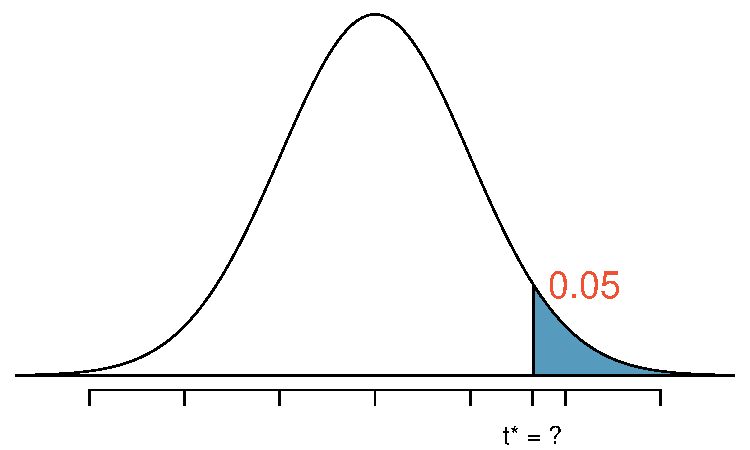
\includegraphics[width=\textwidth]{figures/med_hist_surveys/power_t_star_clicker.pdf}
}

\end{frame}

%%%%%%%%%%%%%%%%%%%%%%%%%%%%%%%%%%%%

\begin{frame}
\frametitle{Problem 1 - cont.}

\clicker{Which values of ($\bar{x}_{new} - \bar{x}_{current}$) represent sufficient 
evidence to reject $H_0$?
\begin{itemize}
\item[] $H_0: \mu_{new} - \mu_{current} = 0$
\item[] $H_A: \mu_{new} - \mu_{current} > 0$
\item[] $n_{new} = n_{current} = 150$, $\alpha = 0.05$, $s_{new} = 2.2 = s_{current} = 2.2$
\end{itemize}
}

\twocol{0.5}{0.5}
{
{\small
\begin{enumerate}[(a)]
\item $\bar{x}_{new} - \bar{x}_{current} < -0.42$
\item $\bar{x}_{new} - \bar{x}_{current} > - 0.42$
\item $\bar{x}_{new} - \bar{x}_{current} < 0.42$
\item \solnMult{$\bar{x}_{new} - \bar{x}_{current} > 0.42$}
\item $\bar{x}_{new} - \bar{x}_{current} > 1.66$
\end{enumerate}
}
}
{
\soln{\pause
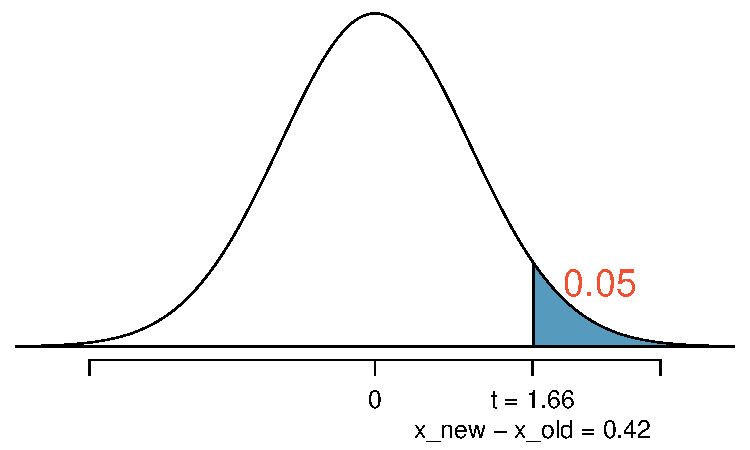
\includegraphics[width=\textwidth]{figures/med_hist_surveys/power_t_star_obs.pdf}
}
}

\end{frame}

%%%%%%%%%%%%%%%%%%%%%%%%%%%%%%%%%%%%

\begin{frame}
\frametitle{Problem 2}

\clicker{What is the probability that we would reject this $H_0$ if $\bar{x}_{new} - \bar{x}_{current}$ 
had come from a distribution with $\mu_{new} - \mu_{current} = 0.5$, i.e. what is the probability that we 
can obtain such an observed difference from this distribution?
\begin{itemize}
\item[] $H_0: \mu_{new} - \mu_{current} = 0$
\item[] $H_A: \mu_{new} - \mu_{current} > 0$
\item[] $n_{new} = n_{current} = 150$, $\alpha = 0.05$, $s_{new} = 2.2 = s_{current} = 2.2$
\end{itemize}
}

\twocol{0.2}{0.8}
{
{\small
\begin{enumerate}[(a)]
\item 5\%
\item 38\%
\item \solnMult{62\%}
\item 80\%
\item 95\%
\end{enumerate}
}
}
{
\soln{\pause
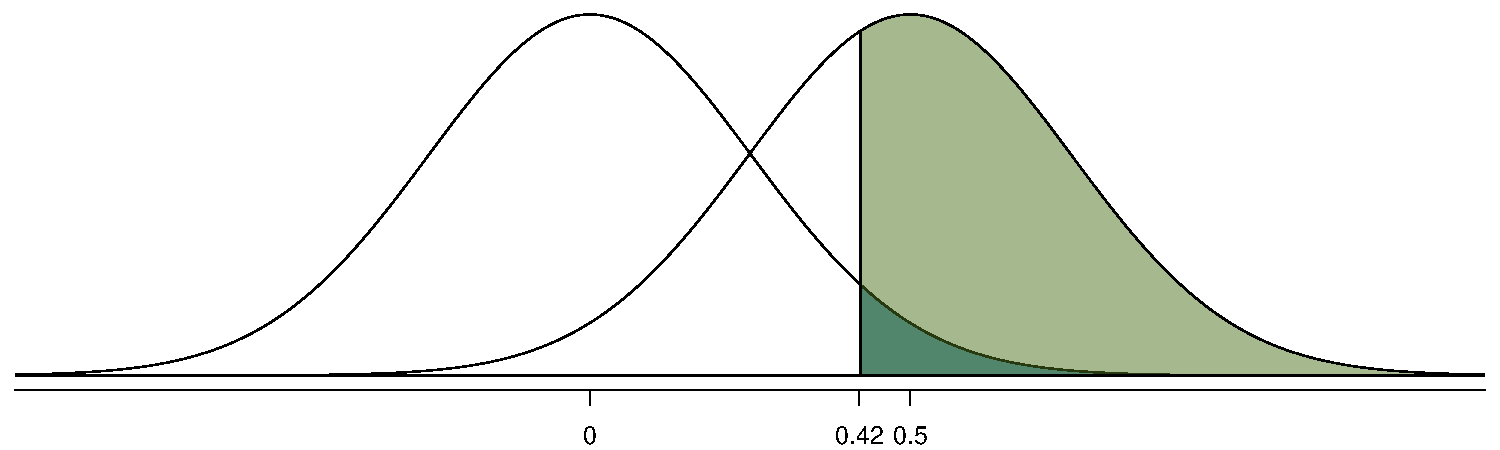
\includegraphics[width=\textwidth]{figures/med_hist_surveys/power.pdf}
}
}

\end{frame}

%%%%%%%%%%%%%%%%%%%%%%%%%%%%%%%%%%%%

\begin{frame}
\frametitle{Problem 2 - cont.}

\clicker{What is $\beta$, the Type 2 error rate?}

\begin{enumerate}[(a)]
\item 5\%
\item \solnMult{38\%}
\item 62\%
\item 80\%
\item 95\%
\end{enumerate}

\end{frame}

%%%%%%%%%%%%%%%%%%%%%%%%%%%%%%%%%%%%

\subsection{Power goes up with effect size and sample size, and is inversely proportional
with significance level and standard error}
\label{mi5}

%%%%%%%%%%%%%%%%%%%%%%%%%%%%%%%%%%%

\begin{frame}
\frametitle{Achieving desired power}

There are several ways to increase power (and hence decrease Type 2 error rate):

\pause

\begin{enumerate}

\item Increase the sample size.

\pause

\item Decrease the standard deviation of the sample, which is equivalent to increasing the 
sample size (it will decrease the standard error). With a smaller $s$ we have a better chance 
of distinguishing the null value from the observed point estimate. This is difficult to ensure but 
cautious measurement process and limiting the population so that it is more homogenous may help.

\pause

\item Increase $\alpha$, which will make it more likely to reject $H_0$ (but note that this has the 
side effect of increasing the Type 1 error rate).

\pause

\item Consider a larger effect size. If the true mean of the population is in the alternative hypothesis 
but close to the null value, it will be harder to detect a difference.

\end{enumerate}

\end{frame}

%%%%%%%%%%%%%%%%%%%%%%%%%%%%%%%%%%%

\begin{frame}
\frametitle{Recap - Calculating Power}

\begin{itemize}

\item \hl{Step 0:} Pick a meaningful effect size $\delta$ and a significance level $\alpha$

~\\

\item \hl{Step 1:} Calculate the range of values for the point estimate beyond which you would reject $H_0$ at the chosen $\alpha$ level.

~\\

\item \hl{Step 2:} Calculate the probability of observing a value from preceding step if the sample was derived from a population where $\mu = \mu_{H_0}+\delta$

\end{itemize}

\end{frame}


%%%%%%%%%%%%%%%%%%%%%%%%%%%%%%%%%%%%

\subsection{A priori power calculations determine desired sample size}
\label{mi6}

%%%%%%%%%%%%%%%%%%%%%%%%%%%%%%%%%%%

\begin{frame}
\frametitle{Back to medical surveys...}

{\small
\disc{How large a sample size would you need if you wanted 90\% power to detect a 0.5 increase
in average number of surveys taken at the 5\% significance level?  \vspace{-3mm}
\begin{itemize}
\item[] $H_0: \mu_{new} - \mu_{current} = 0$, $H_A: \mu_{new} - \mu_{current} > 0$ \vspace{-3mm}
\item[] $n_{new} = n_{current} = ?$, $s_{new} = 2.2 = s_{current} = 2.2$ \vspace{-3mm}
\item[] $\delta = 0.5$, $\alpha = 0.05$, power = 90\%, $\beta = 0.10$ \vspace{-1mm}
\end{itemize}
}}

\pause

\begin{center}
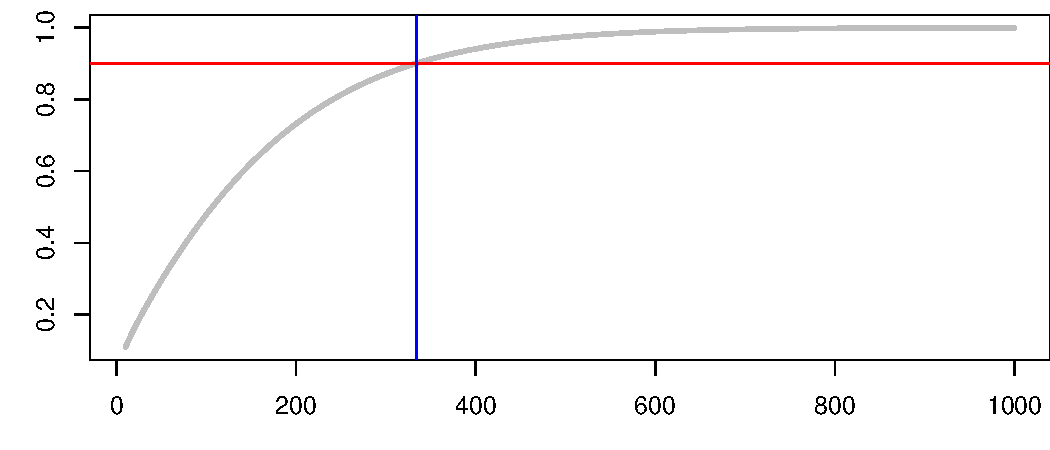
\includegraphics[width=0.7\textwidth]{figures/med_hist_surveys/power_curve.pdf}
\end{center}

When $n > 334$, power is at least 90\%.

\end{frame}

%%%%%%%%%%%%%%%%%%%%%%%%%%%%%%%%%%%%%

\begin{frame}[fragile]
\frametitle{If you're interested...}

{\scriptsize
\begin{verbatim}
s = 2.2
mu = 0
delta = 0.5

ns = 10:1000
power = rep(NA, length(ns))

for(i in 10:1000){
  n = i
  t_star = qt(0.95, df = n-1)
  se = sqrt((s^2 / n) + (s^2 / n))
  cutoff = t_star * se
  t_cutoff = (cutoff - (mu+delta)) / se
  power[i-9] = pt(t_cutoff, df = n-1, lower.tail = FALSE)
}

which_n = which.min(abs(power - 0.9))
power[which_n]
power[which_n + 1]
ns[which_n + 1]
\end{verbatim}
}

\end{frame}

%%%%%%%%%%%%%%%%%%%%%%%%%%%%%%%%%%%%%

\begin{frame}

\vfill

\app{4.3}{See course website for details.}

\vfill

\end{frame}

%%%%%%%%%%%%%%%%%%%%%%%%%%%%%%%%%%%%

\section{Summary}

%%%%%%%%%%%%%%%%%%%%%%%%%%%%%%%%%%%

\begin{frame}
\frametitle{Summary of main ideas}

\vfill

\begin{enumerate}

\item \nameref{mi1}

\item \nameref{mi2}

\item \nameref{mi3}

\item \nameref{mi4}

\item \nameref{mi5}

\item \nameref{mi6}

\end{enumerate}

\vfill

\end{frame}

%%%%%%%%%%%%%%%%%%%%%%%%%%%%%%%%%%%

\end{document}